%!TEX TS-program = xelatex
%!TEX encoding = UTF-8 Unicode


\documentclass[utf8]{XDBAthesis}

\def\allfiles{}
%\usepackage{indentfirst} %首行缩进
%\usepackage{amsmath}%换行
%\usepackage{ctex}
%\usepackage{amsfonts, amssymb}%数学字体
%\usepackage{tikz}%绘图
%\usepackage{subfigure}
%\usepackage{graphicx}
%\usepackage{caption}
%\makeatletter
%\newcommand\figcaption{\def\@captype{figure}\caption} 
%\newcommand\tabcaption{\def\@captype{table}\caption}
%\renewcommand\figurename{图} 
%\makeatother
%\usepackage{float}
%\usepackage[bookmarksnumbered]{hyperref}
%
%

\begin{document}
    \class{031111}
    \schoolnumber{03111002}
    \title{翻译:G-Hash}{}   %%题目超过14个字把剩下的放到第二个空
    \college{计算机学院}
    \major{计算机科学与技术}
    \author{贾新禹}
    \advisor{霍红卫}
    \maketitle
\tableofcontents

\ifx\allfiles\undefined
\documentclass{article}
\usepackage{amsmath}%换行
\usepackage{ctex}
\usepackage{tikz}
\usepackage{subfigure}
\usepackage{graphicx}
\usepackage{caption}
\usepackage{amsfonts, amssymb}%数学字体

\usepackage{indentfirst} %首行缩进
\makeatletter
\newcommand\figcaption{\def\@captype{figure}\caption} 
\newcommand\tabcaption{\def\@captype{table}\caption}
\renewcommand\figurename{图表} 
\makeatother
\usepackage{float}

\begin{document}

\else

\fi
\begin{abstract}
    目前,集合,列表,树和图之类的结构化数据给数据管理这一基础领域提出了一个严峻的挑战。如何对图数据有效存储,索引,搜索都面临着一系列问题。随着图数据库的快速增多,图相似性搜索成为了一个热门的话题。图相似性搜索在多个领域都有应用,像化学结构,分子结构,传感器网络,XML文档等等。
    
    现在大多的图搜索算法都是为了解决精确搜索的,即找到一组包含精确查询图的图集合。因此,我们不能直接利用这些算法进行相似性搜索。在数据挖掘和机器学习领域有很多图核函数来判断图之间的固有相似度,但在图相似性搜索上却很罕见。因为尽管图核函数对于监督学习领域的准确预测和分类模型效果很好,但是用于图相似度查询则会存在两个关键问题:(i)计算复杂度非常高(ii)在图搜索上的应用复杂度也是非平凡的。
    
    而本文中,我们打算利用图核函数进行相似性搜索。为此,我们提出了两个关键概念(i)一种新的图相似度度量方法(ii)一种新的图数据索引策略。我们以每个节点和其邻接节点特征为相似性度量依据,并利用哈希表来进行高效存储和快速查询。我们这种利用图核函数抓住图相似性的本质特征,并利用哈希表加速查询过程的新算法,我们称之为G-Hash。本文中我们详细介绍了这种方法,并在大规模的化学结构数据库上进行了实验。结果表明G-Hash在k个最相近邻居问题上已经达到了业界的最高水平,更重要的是,我们这种新的相似性度量方法和索引结构比现有的算法(C-tree,gIndex,GraphGrep等)具有更小的索引尺寸和更快的查询速度。
    
    \textbf{关键词:图相似性搜索,图分类,哈希,图核,k-NNs查询}
\end{abstract}

\ifx\allfiles\undefined
%\renewcommand\refname{参考文献}
%\bibliographystyle{unsrt}
%\bibliography{G-Hash翻译}
\end{document}
\fi

\ifx\allfiles\undefined
\documentclass{article}
\usepackage{amsmath}%换行
\usepackage{ctex}
\usepackage{tikz}
\usepackage{subfigure}
\usepackage{graphicx}
\usepackage{caption}
\usepackage{amsfonts, amssymb}%数学字体

\usepackage{indentfirst} %首行缩进
\makeatletter
\newcommand\figcaption{\def\@captype{figure}\caption} 
\newcommand\tabcaption{\def\@captype{table}\caption}
\renewcommand\figurename{图表} 
\makeatother
\usepackage{float}

\begin{document}

\else

\fi
\chapter{引言}
目前,形如集合,序列,树和图等结构化数据给像高效存储,索引,部分查询(如子图/超图搜索)和相似性搜索之类的传统数据管理领域提出了一个巨大的挑战。随着图数据库的迅速发展,在图数据库中的\emph{图相似性搜索}成为了一个日益重要的研究课题。图相似性搜索已经多个领域进行了应用,例如化学,分子信息学,传感器网络管理,社交网络管理,XML文档等等。在化学与制药领域,每天会产生大量的化学分子结构数据。一旦一个新的化学结构被合成后,这个结构的特性就可能通过查询已知的分子结构,通过其特性来预测。大规模图数据中的相似性搜索让科研人员和工程师们可以对图精确建模,认识到图数据间的固有联系,减少大数据库的计算代价。

图查询需要分成两种:(i)子图查询(ii)相似度查询。\emph{子图查询}目的是确定一个包含着查询图的集合。\emph{相似性查询}是根据差异距离来找出数据库中和查询相似的图,如$k$-NNs查询(最相近$k$查询)和范围查询。$k$-NNs查询是为了得到最相近的$k$个图。范围查询,是为了得到差异距离小于预设值的所有图。在本文中,我们只研究在大规模图数据库中的$k$-NNs相似性搜索。

在图上进行相似性搜索是十分富有挑战的。我们认为一个理想相似性搜索设计应该达到以下三个相关的(有时是相反的)目标:准确度高,时间短,空间小。为了准确度高,我们要求相似性度量方法应该抓住数据的固有相似度。众所周知,一些图上的操作,像子图同构,都是NP问题。所以为了时间短,我们需要设计一个高效的算法来尽量避免全图搜索。为了空间小,所以索引结构不能对图数据库开销太大。

许多简单的图相似性度量方法是将图转换为在高维欧几里得空间(\emph{特征空间})中的表示,然后利用空间上的索引技术来进行相似度搜索。现有的特征提取方法大多数都可以归为两类:(i)每幅图的子结构单独计数(如从一幅图中生成随机的通路),(ii)图集合中的子结构一起计数(如挖掘频繁子结构)。尽管相似性搜索已经被广泛应用了,但是在特征提取的适配性和特征的索引策略上仍有很多限制。首先,图数据库(尤其是大规模的图数据库)的特征提取是需要大量运算量的。其次,特征提取过程可能产生很多特征值,需要占用大量内存空间。学术界曾提出过许多不同的特征选取方法来确定“有辨识度的”特征。但是,对于数据库搜索表现优异的特征选取方法在图相似性上不一定会很好,所以我们还需要自行去判断与权衡。

在本文中,我们探索了一种新的图相似性搜索方法。我们通过核函数来定义相似度。和通常不同的是,\emph{核函数}没有直接提取特征值,而是将数据映射到一个高维的函数空间,并利用在这个函数空间中数据的内积来计算其相似度。基于核函数的图相似度测量方法的优势在于核函数统计学表现非常好,例如可以高精度的分类。但是将核函数用于数据库搜索也有些问题,主要的难点在于(i)核函数用在图上计算量很大(ii)目前为止,没有一个明确的方法来标引大规模图数据库上的核函数计算。

我们的方法称作G-hash。我们致力于提出一种新的核函数来高效计算大规模图数据库上的特征。在我们的模型中,图被用核函数直接压缩成一个节点集。传统上,对于复杂的图结构,这样的压缩方法会丢失大量的信息。但是我们将大多数拓扑信息压缩到了每个节点的特征向量上来避免大量信息的丢失。这种方法提供了一个对于信息量丰富的图的简单表示,并且也很好进行比较。我们接着利用压缩集表示法将图节点哈希化。哈希的键值是基于这些表示集的,所以相似的节点会被哈希到同一个格子或者相邻的格子中。一旦我们将数据库中所有图哈希成一个表后,我们可以找到所有相似的节点,然后利用它们计算查询图和数据库中图的距离,并找出查询图的$k$-NNs(k个相近图)。

总体而言,我们这篇文章的主要贡献有:
\begin{itemize}
    \item 提出了一个图核函数和用来进行快速图相似性搜索的索引结构
    \item 我们的索引只需线性时间去计算(对数据库中的总结点数而言),并且可以通过动态增删来在线构建。
    \item 我们证明了新的图核函数和相应的索引结构可以更好地在抓取固有图相似性和对于大数据库的快速计算上平衡。
\end{itemize}
本文组织如下,我们首先在第二章回顾了一些相关领域,如哈希,索引,图核函数等等。在第三章,我们正式定义了图和图相似性搜索。在第四章我们讨论了索引结构和核函数的细节。最后我们对我们的算法进行了广泛的实验,并与现有算法进行对比,并得出了一些结论来指导我们的研究。




\ifx\allfiles\undefined
%\renewcommand\refname{参考文献}
%\bibliographystyle{unsrt}
%\bibliography{G-Hash翻译}
\end{document}
\fi
\ifx\allfiles\undefined
\documentclass{article}
\usepackage{amsmath}%换行
\usepackage{ctex}
\usepackage{tikz}
\usepackage{subfigure}
\usepackage{graphicx}
\usepackage{caption}
\usepackage{amsfonts, amssymb}%数学字体

\usepackage{indentfirst} %首行缩进
\makeatletter
\newcommand\figcaption{\def\@captype{figure}\caption} 
\newcommand\tabcaption{\def\@captype{table}\caption}
\renewcommand\figurename{图表} 
\makeatother
\usepackage{float}

\begin{document}

\else

\fi
\chapter{相关研究 \\ Related Work}
在本章中,我们讨论一些相关的研究。从基本的图数据库索引,子图搜索,模糊子图搜索和图相似性搜索到图核函数
\section{子图搜索 \\ Subgraph Search}
现在许多的子图搜索都采用了一个相似的框架,先把图分解为一系列小片段,然后将其作为特征,并基于其建立基于特征的索引结构来进行子图查询。属于这类的方法有\emph{GraphGrep,gIndex,FG-Index,Tree+Delta}和\emph{GDIndex}。

在图索引中,最简单的特征就是通路(walk)。一些情况下,我们可以用路径作为特征,就像这个领域的先驱方法\emph{GraphGrep}.路径很好检索特性,并且很好处理。但是,路径的简单性却制约着这种方法的性能。举例而言,即便两图的所有路径都是不同长度的,我们利用路径也不能区分出环和链的拓扑结构。

当意识到路径的局限性后,\emph{gIndex}和\emph{FG-Index}便应运而生了。这两种方法利用子图结构来有效分辨路径和环。但是,基于子图结构的索引也有一些限制,就是子图的枚举和匹配都是运算量非常大的过程。为了克服这些障碍,这些方法采用只提取\emph{频繁子结构}来作为索引特征。还有些相似的方法,像\emph{Tree+Delta}和\emph{TreePi}则用频繁树结构来代替频繁子图结构来克服这些障碍。

\emph{GDIndex}也采用子图结构算法作为基本索引特征,但是并不使其局限于\emph{频繁}子图结构,除此之外,这个算法还采用了哈希表来加速图同构查询。尽管这个算法设计目的是为了子图查询,但也同样支持相似查询。

\section{模糊子图搜索 \\ Approximate Subgraph Search}
除了精确图匹配,也有些其他算法放宽了同构的限时,允许部分匹配或者模糊匹配。这是一个相对较新的领域,因此并没有太多的算法针对这个问题。有一个针对这个问题的算法,\emph{SAGA},它被设计用来作为生物路径分析。首先,建立一个基于图片段的索引。当候选图与查询图失配时,我们用一个图距离度量方法来度量差异。

另一个算法叫做\emph{gApprox}和\emph{gIndex}相似。从思想到名字,包括作者都很相似。这种算法力求从数据库中挖掘频繁\emph{模糊}模式,并以此作为索引特征。他们还提出一个概念,称为\emph{模糊频繁}。

TALE算法也是用来做模糊匹配的一种算法。但是它着重于处理有上千节点的大图。


\section{图相似性搜索 \\ Graph Similarity Search}
通常,我们有很多方法去测量图之间的相似度。第一种方法是\emph{编辑距离(edit distance)}.\emph{编辑距离}就是我们将图$G$通过一系列操作(增删点边,重新标号等)变换为另一个图$G^{'}$所需的操作数。我们可以通过给不同操作分配不同的费用,然后用费用总和当做距离来调整这个方法的准确度。虽然编辑距离是一种非常直观的图相似性测度方法,但是实际上我们难以计算它(是个NP-hard问题).\emph{C-Tree}\cite{C-Tree}是一种被广泛使用的图索引模型。它没有使用图的片段信息作为特征值,而是把数据图组织在一种内部节点是\emph{图闭包(graph closures)},叶节点是数据图的树形结构中。相比于前两种方法\emph{GraphGrep}和\emph{gIndex},\emph{C-Tree}的最大优势在于其支持相似性搜索,而前两个并不支持。

还有一种名为\emph{GString}的子图相似性查询方法也和\emph{GraphGrep}一样是用图片段作为特征值的。当然,这种方法与前面两种基于特征值的子图查询还是不同的。在这个方法中,首先我们分解复杂图为节点数较少的连通图,得到的这些连通图每个都是一个特定的图片段。随后,我们用一种标准的编号方式把数据库中的所有图都转化为一个个字符串。并用这些字符串构建一颗后缀树来支持相似性搜索。这种方法融合了子图的数据表达能力(信息完整)和用字符串匹配来查询图的速度(速度快)。

另外,\emph{最大公共子图(maximal common subgraph)}\cite{mcs}和\emph{图配对(graph alignment)}\cite{assignment,assigment08} 这两种方法也常被用来定义图相似度。虽然有这么多方法,但是不幸的是迄今为止我们仍没有一种简单的方法来索引或者度量大图数据库。

\section{图核函数 \\ Graph Kernel Functions}
目前业界有很多图核函数,而开创性的一个图核函数是Haussler在他对\emph{R卷积核(R-convolution kernel)}的研究中提出的。现在大多数图核函数都遵循它提出的这种框架。R卷积核是基于把离散的结构(如图)分解成一系列的组成元素(子图)这个思想的。我们可以定义许多这样的分解,就像组成结构中的核心一样。R卷积核保证无论选择怎样的分解方式或者结构核心,都能得要一个对称半正定的函数,或者一个结构间的核函数。这个关键性质将寻找离散结构核函数的问题简化为寻找分解方式和结构间的核函数。R卷积核可以通过加权分解核来允许组件结构间的加权核。

目前图核函数的研究可以大致分为两类:第一类是考虑图中的所有可能组成结构(例如所有路径),然后以此来计算两图之间的相似度。这一类的算法有product graph kernel,random walk based kernel和基于点对间最短路径的核。第二类核函数是尝试通过一组特殊的(有限的)结构来计算局部相似度,并且值在这有限的结构中统计共享的结构。这种方法包含一大类图核算法,叫做spectrum核,还有最近频繁子图核。我们发现最有效的核函数是Vishwanathan提出的用于全局相似性度量的方法。全局度量需要$O(n^3 )$的时间复杂度,$n$是图中最大的节点数。众所周知,不同于全局相似度测量,局部相似性度量时间代价是非常昂贵的。因为子结构匹配(如子图同构)是一个NP-hard的问题。

我们采用一个最近提出的图小波匹配核,并将其扩展使其能在大数据库运行。

\ifx\allfiles\undefined
%\renewcommand\refname{参考文献}
%\bibliographystyle{unsrt}
%\bibliography{G-Hash翻译}
\end{document}
\fi
\ifx\allfiles\undefined
\documentclass{article}
\usepackage{amsmath}%换行
\usepackage{ctex}
\usepackage{tikz}
\usepackage{subfigure}
\usepackage{graphicx}
\usepackage{caption}
\usepackage{amsfonts, amssymb}%数学字体

\usepackage{indentfirst} %首行缩进
\makeatletter
\newcommand\figcaption{\def\@captype{figure}\caption} 
\newcommand\tabcaption{\def\@captype{table}\caption}
\renewcommand\figurename{图表} 
\makeatother
\usepackage{float}


\begin{document}
\else
\fi
\chapter{背景知识 \\ Background}
在我们详细介绍算法细节之前,让我们先了解一下关于图分析计算的所需的基本背景。这章包含(i)图核函数,(ii)图小波分析两部分。
\section{图 \\ Graphs}
一个\emph{标号图}可以被一个有限的节点集合$V$和一个有限的边集合$E\in V\times V$所描述。在大多数应用中,图都是有标号的。这些标号都是从一个标号集选取的,我们用一个标号函数$\lambda :V\cup E\rightarrow \Sigma$来给各个节点和边分配标号。在\emph{标号点图}中只有点有标号,同样,在\emph{标号边图}中只有边有标号。在\emph{全标号图}中,边点都有标号。如果用一种特殊的标号来表示未标号的点和边,那么标号点图和标号边图都可以被看做是全标号图的特殊形式。所以在此文中我们只考虑全标号图来简化问题而又不失一般性。对于标号集$\Sigma$我们并不指定具体结构,可以是一个字段,一个向量,也可以是很简单的是个集合。
以下我们约定,一幅图用一个四元组$G=(V,E,\Sigma ,\lambda )$表示,$V,E,\Sigma,\lambda$都如上文所述。如果一幅图$G=(V,E,\Sigma,\lambda)$和另一幅图$G'=(V',E',\Sigma',\lambda')$有1-1映射的关系$f:V\rightarrow V'$,那么图$G$就是$G'$的\emph{子图},用$G\in G' $表示。1-1映射可以有这么几种
\begin{itemize}
    \item 对于所有$v\in V,\lambda(v)=\lambda '(f(v))$
    \item 对于所有$(u,v)\in E,(f(u),f(v))\in E'$
    \item 对于所有$(u,v)\in E,\lambda(u,v)=\lambda '(f(u),f(v)) $
\end{itemize}
换言之,如果一幅图保持着另一幅图的所节点标签,边关系,和边标签,那么这副图就是另一幅图的子图。
一个\emph{通路(walk)}是一个节点列表$v_1,v_2,...,v_n$,对于所有$i\in [1,n-1]$,$v_i$和$v_{i+1}$有边连接。一个\emph{路径(path)}是一个不含重复节点的通路,即对于所有$i\neq j,v_i \neq v_j$。
\section{再生核Hilbert空间 \\ Reproducing Kernel Hilbert Space}
对于大量图数据的分析,核函数是一个很强大的处理工具。核函数的优势在于它无需精确计算对应点对就可以把一组数据放入一个高维的Hibert空间。我们用一个叫做\emph{核}的函数来处理这个过程。
一个二元函数$K:X\times X\rightarrow \mathbb{R}$ 如果符合以下公式,则它是一个\emph{半正定}函数。
\begin{equation}
    \sum_{i,j=1}^{m}c_i c_j K(x_i ,x_j )\geq 0
\end{equation}
上式中$m\in \mathbb{N}$,例子$x_i \in X(i=[1,n])$,系数集$c_i \in \mathbb{R}(i=[1,n])$。另外,如果$对于所有x,y\in 都有X,K(x,y)=K(y,x)$那么这个二元函数就是\emph{对称的}。一个对称半正定函数保证存在一个Hilbert空间$\mathcal{H}$和一个映射$\Phi:X\rightarrow \mathcal{H} $,例如
\begin{equation}
    k(x,x')=\langle\Phi(x),\Phi(x')\rangle
\end{equation}
对于所有的$x,x'\in X $。$\langle x,y\rangle$表示$x$与$y$的内积。这个结果就是我们所熟悉的Mercer定理。一个对称半正定函数又称为Mercer核函数简称为\emph{核}函数。
通过将数据空间变为Hilbert空间,核函数提供了一种对包括图在内的不同数据的统一分析环境。即使一开始的数据空间根本不像一个向量空间,也可以统一化。我们称这种归一化方法为"核诀窍",并将其应用在许多不同的数据分析任务上,包括分类,回归,通过准则分析的特征提取等。
\section{图小波分析 \\ Graph Wavelets Analysis}
小波函数常被当做一种用于将一个函数或者信号通过不同的变换分解和表示为它的子结构的方法。小波常用在数字化的数据上,例如通信信号或者数学函数,也可以用在一些规律的数值结构上,像矩阵和图像。但是图是一种随意的结构,并且可能表示非数值化的关系,在数据元素之间也可能存在拓扑关系。近期的一些研究证实了利用小波函数对图做多解析度分析的可行性。两个小波函数的典型就是$Haar$和$Mexican hat$。
Crovella和其他人开发了一种对于交通网络数据分析的多尺度方法。在这个应用中,他们尝试去确定一个交通现象发生的规模。他们将交通网络表示为一个标号图,并且用一些测量方法像每个单位时间的比特携带数来做标号。
Maggioni和其同事证实了一个通用的双正小波分析可用于图分析。在他们的方法中,他们将利用扩散操作的二元性来激发多解析度分析。他们的方法主要适用于大空间的分类,例如流形和图,对于带属性的分子结构的适应性尚不清楚。在这里主要的技术问题就是如何在多解析度分析中包含节点标签。


\ifx\allfiles\undefined
%\renewcommand\refname{参考文献}
%\bibliographystyle{unsrt}
%\bibliography{G-Hash翻译}
\end{document}
\fi
\ifx\allfiles\undefined
\documentclass{article}
\usepackage{amsmath}%换行
\usepackage{ctex}
\usepackage{tikz}
\usepackage{subfigure}
\usepackage{graphicx}
\usepackage{caption}
\usepackage{amsfonts, amssymb}%数学字体

\usepackage{indentfirst} %首行缩进
\makeatletter
\newcommand\figcaption{\def\@captype{figure}\caption} 
\newcommand\tabcaption{\def\@captype{table}\caption}
\renewcommand\figurename{图表} 
\makeatother
\usepackage{float}

\begin{document}

\else

\fi
\section{基于哈希的快速图相似性搜索}
正如之前所说,现在的图查询算法查询时间很快但是没有好的相似性度量方法。核函数可以提供一个好的相似性度量方法,但是核函数的矩阵运算需要大量的时间,所以我们很难直接利用其来建立索引。为了解决这个问题,我们提出了一种新的算法,G-Hash。现在的算法常常关注速度或精度的一种,而G-Hash在两者效果均很好。我们利用小波图匹配核(WA)来定义相似性,并用Hash表作为索引结构来加速图相似性查询。下面我们先介绍下WA方法。

\ifx\allfiles\undefined
%\renewcommand\refname{参考文献}
%\bibliographystyle{unsrt}
%\bibliography{G-Hash翻译}
\end{document}
\fi
\ifx\allfiles\undefined
\documentclass{article}
\usepackage{amsmath}%换行
\usepackage{ctex}
\usepackage{tikz}
\usepackage{subfigure}
\usepackage{graphicx}
\usepackage{caption}
\usepackage{indentfirst} %首行缩进
\makeatletter
\newcommand\figcaption{\def\@captype{figure}\caption} 
\newcommand\tabcaption{\def\@captype{table}\caption}
\renewcommand\figurename{图表} 
\makeatother
\usepackage{float}


\begin{document}
\section{Hash函数实现快速图相似性搜索}
\else
\subsection{Hash函数实现快速图相似性搜索}
\fi
根据将图中的每个节点利用函数映射到一个特征空间上的这一思想,我们可以设计出一种核函数来进行快速相似性搜索。具体的说,我们有了以下两条发现。
\begin{itemize}
    \item 当图$G$中节点$u$向量和图$G'$中的节点$v$完全不同,节点$u$和$v$的核值很小基本不影响图核值。所以我们如果仅计算相似点对的核值,得到的核矩阵将和WA方法中的相似性度量类似,但耗时很少。
    \item 如果基于节点向量来构造哈希表的话,相似的对象的位置上将也很靠近。所以我们可以很快速得利用哈希表来寻找相似点对。另外,如果数据库中所有图都存入哈希表中的话,一个位置可能对应不同图中的多个相似节点。因为这些节点都是相似的,所以只要利用其中两个节点进行一次RBF核运算就可以代表所有的结果了。节点覆盖给了我们另一个省时间的契机。
\end{itemize}

基于以上两条发现,我们引入我们的方法:\emph{k}-NNs查询(G-hash).G-Hash是一种利用WA方法进行精确相似度度量,并利用哈希来降低时间复杂度。具体算法见下文。

\subsection{索引构建}
像WA方法一样,我们首先需要利用小波变换将数据库中的所有图拆解成点向量的形式。因为WA方法对距离参数的选取并不敏感,用不同的小波算法造成的差异也并不大\cite{Graph_wavelet} ,所以我们设定\emph{h}为2,并才用\emph{Haar}小波算法来简化算法

当图完全拆解成节点向量后,我们就可以利用这些向量构建哈希表。这时,我们需要一个哈希函数来把相似的节点哈希到相同的位置。这就意味着我们要基于节点向量构建哈希键。我们可以用和构造节点向量同样的思想构建哈希键,即利用节点标号和邻接信息来构造。我们将每一个节点向量中的特征信息离散成一个整数,并将每个节点标签直接编码为一个n位的字符串(除去一个代表本身标号的1,其他全0)。其他特征就近似到最近的整数上。当节点向量变成了一个整数列表后,我们再把节点向量变为一个字符串(用二进制表示每个整数,并用下划线连接)。这样的一个字符串就是对于节点的哈希键。我们以图表1的图P来举例说明。


\tikzstyle{vertex}=[circle,fill=black!25,minimum size=20pt,inner sep=0pt]
\tikzstyle{selected vertex} = [vertex, fill=red!24]
\tikzstyle{edge} = [draw,thick,-]
\begin{figure}[H]
\begin{minipage}{\textwidth}
例子 4.1. \emph{我们选取节点标签和邻接节点各个标号的个数作为度量特征。所以我们一共有四个特征。这个图的特征仅属于取值中的一种:nominal。我们首先写出节点特征矩阵如图表1中的(B)。然后用小波函数提取出实际特征值。举例而言,对于$P_{3}$在用$h=0$的小波分析提取后,局部特征是$\lbrack b,2,0,1\rbrack $。然后生成的哈希表如图表1(C)所示。}  \\ \\
\end{minipage} 
\subfigure[P]{   
\begin{minipage}{0.5\textwidth}
    \centering
    \begin{tikzpicture}[scale=1.1, auto,swap]
        \foreach \pos/\labels/\name in {{(0,1)/1/a}, {(1,2)/2/a}, {(1,0)/3/b},{(3,0)/4/c}, {(3,2)/5/c}}
            \node[vertex] (\labels) at \pos [label=above:$P_{\labels}$]{$\name$};
        \foreach \source/ \dest  in {1/2,1/3,1/3,2/5,3/4}
                \path[edge] (\source) --  (\dest);
    \end{tikzpicture}
\end{minipage}
}
\subfigure[节点特征矩阵]{
\begin{minipage}{0.5\textwidth}
    \centering
    \begin{tabular}{c|c|c|c|c}
        Nodes & Label & \#a & \#b & \#c \\ \hline
        $P_{1}$ & a & 1 & 1 & 0 \\ \hline
        $P_{2}$ & a & 1 & 1 & 1 \\ \hline
        $P_{3}$ & b & 2 & 0 & 1 \\ \hline
        $P_{4}$ & c & 0 & 1 & 0 \\ \hline
        $P_{5}$ & c & 1 & 0 & 0 \\ \hline
    \end{tabular}
\end{minipage}
}
\subfigure[图P的哈希表]{
\begin{minipage}{\textwidth}
    \centering
    \begin{tabular}{c|c}
        哈希键 & 哈希值  \\ \hline
        a,1,1,0 & $P_{1}$ \\ \hline
        a,1,1,1 & $P_{2}$ \\ \hline
        b,2,0,1 & $P_{3}$ \\ \hline
        c,0,1,0 & $P_{4}$ \\ \hline
        a,1,1,1 & $P_{5}$ \\ \hline
    \end{tabular}
\end{minipage}
}
\caption{一幅简单图}
\end{figure}

注意:在这个算法框架中,我们在构建哈希索引时没有对查询图做任何假设。



\subsection{\emph{K-NNs}查询过程}
为了获得对于给定图的\emph{K-NNs},我们需要计算它和数据库中其他图的距离。以下是我们定义的利用核函数进行两图距离度量的函数
\begin{equation}
\begin{split}
    &d(G,G')=\sqrt{\|\phi(G)-\phi(G')\|_{2}^{2}}\\
              &=\sqrt{\langle\phi(G)-\phi(G'),\phi(G)-\phi(G')\rangle}\\
              &=\sqrt{\langle\phi(G),\phi(G)\rangle+\langle\phi(G'),\phi(G')\rangle-2\langle\phi(G),\phi(G')\rangle}\\
              &=\sqrt{k_{m}(G,G)+k_{m}(G',G')-2k_{m}(G,G')}
\end{split}
\end{equation}

公式中$k_{m}(G,G)$代表图$G$和其本身的核函数值,$k_{m}(G',G')$是图$G'$及其本身的值,$k_{m}(G,G')$就是图$G$和$G'$的。在后文中,我们会介绍该如何计算这些值。

尽管在将查询图节点哈希到哈希表时,我们可以得到核函数
\begin{equation}
k_{m}(G,G')=\sum_{v\in G',u\in simi(v)}K(\Gamma^{h}(u),\Gamma^{h}(v))
\end{equation}

$simi(v)$是一个包含着图$G$和节点$v$哈希到同一个位置的节点集合。我们用以下的解码方式来获取包含这些节点的图号和节点号。

显然,仅利用相似点对而非所有点对来计算两图相似度可以节约很多运算时间。因此为了增加准确度,相似的节点应该被哈希到相邻的位置。在图很大(如大于40)时,我们也要计算相邻位置的节点。

因此在核函数计算时我们只考虑相似点对,在使用RBF核的情况下,$K(\Gamma^{h}(u),\Gamma^{h}(v))\approx1$,所以公式(2)可以写成
\begin{equation}
    K(G,G')\approx\sum_{v\in G',u\in simi(v)}1=\sum_{v\in G'}|simi(v)| 
\end{equation}

$|simi(v)|$是在$simi(v)$中的节点数目。这意味着我们只需要统计图$G$中和查询$G'$相似的点个数,其和就是我们要求的核。同理,我们可以这样计算每个图与其自己的核。

在完成上述操作后,我们会得到一个距离向量,其每一个值都对应这一个数据库中的图与查询图的距离,通过对这个距离向量排序,我们就可以得到对于给定的查询的$K-NNs$。

\subsection{动态插入与删除}
如果要向数据库中插入一副图,我们只需将新图的节点进行哈希,然后加入节点哈希表。这样插入完成后,只有图中所有的节点的位置会发生变化。而且,因为一幅图的节点是有限的,所以插入操作的时间和构建索引的内存也是有限的。删除操作和插入类似,我们只需找到图中节点在哈希表中的对应哈希值,然后删掉即可。

\ifx\allfiles\undefined
\renewcommand\refname{参考文献}
\bibliographystyle{unsrt}
\bibliography{G-Hash翻译}
\end{document}
\fi
\ifx\allfiles\undefined
\documentclass{article}
\usepackage{amsmath}%换行
\usepackage{ctex}
\usepackage{tikz}
\usepackage{subfigure}
\usepackage{graphicx}
\usepackage{caption}
\usepackage{amsfonts, amssymb}%数学字体

\usepackage{indentfirst} %首行缩进
\makeatletter
\newcommand\figcaption{\def\@captype{figure}\caption} 
\newcommand\tabcaption{\def\@captype{table}\caption}
\renewcommand\figurename{图表} 
\makeatother
\usepackage{float}

\begin{document}

\else

\fi
\chapter{实验研究 \\ Experimental Study}
我们对我们的算法进行了广泛的实验研究来评估其有效性,高效性及扩展性。我们在化学分子结构上测试我们的算法。对于化学结构,节点特征包括数值特征和原子布尔特征。数值特征包括元素种类,原子部分电荷,原子电子亲和势,原子自由电子数目和原子价态等等。布尔特征包括原子是否在供体中,是否在末端碳中,是否在环中,是否为负,是否是轴向的等等。在实验中,我们仅用一个原子特征:元素种类。

我们将我们的方法和小波分配核,C-tree,GraphGrep还有gIndex进行比对。我们的算法,WA算法,GraphGrep和gIndex是基于C++实现的,用g++进行编译。C-tree是用Java实现的,用Sun JDK 1.5.0编译。所有的实验都是在Intel Xeon EM64T 3.2GHz,4G内存,Linux系统这一平台上测试的。

WA,G-Hash,C-tree,GraphGrep和gIndex的参数是这样设置的。对于WA和G-hash,h取2,用\emph{haar}小波函数,对于C-tree,用默认值即将最小子节点数m设为20,最大M设为$2m-1$,用NBM方法进行图映射。对于GraphGrep和gIndex,全部采用默认参数。

\section{数据集 \\ Data Sets}
我们选用许多数据集来进行试验。前五个数据集是从从Jorisson/Gilson数据集获得的已有数据。接下来六个是从BindingDB数据集中抽取的,最后一个是NCI/NIH 艾滋病筛选集里的,表1显示了这些数据集和其基本情况。
\subsection{Jorissen数据集}
Jorissen数据集主要为一些包含活动蛋白质的的化学结构信息。我们以药物对特定蛋白质的吸引力作为的目标值。我们选取了5个包含100个分子结构的蛋白质作为测试目标,其中50个化学结构连接着蛋白质,另外50个没连接到蛋白质上。参考文献14来查看详细信息。

\subsection{NCI/NIH AIDS抗体数据库}
NCI/NIH艾滋病抗体数据库包含42390个化学结构,总共有63种分子,最常见的是,C,O,N,S。数据集包括三种边,单边,双边,芬香边。我们选取了所有结构作为数据库,并随机选取1000个化学结构作为查询集合。
\section{利用分类做节点相似性度量 \\ Similarity Measurement Evaluation with Classification}
我们用不同的相似性度量方法比较\emph{k}-NN分类器在Jorissen数据集和BindingDB数据集上的分类精确度。对于WA算法,我们采用小波匹配核函数来获得核矩阵,然后计算距离矩阵来获得最近的k个最相似的图。对于G-Hash,我们根据之前描述的算法计算核函数,然后找出最相似的k个图。对于C-tree,我们直接找回最相似的子图。我们用标准的5-fold交叉验证来获得分类准确度,$(TP+TN)/S$,其中$TP$表示真正结果的数目,$TN$表示真负的数目,$S$是全部的数据图数目。在本实验中,我们取$k=5$。

\begin{figure}[!htb]
    \centering
    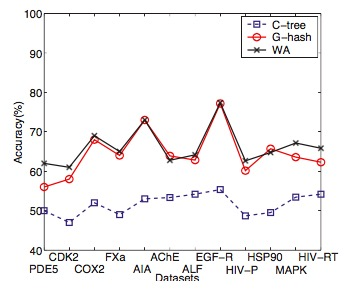
\includegraphics[width=0.5\textwidth]{ac}
    \caption{精确性对比图}
    \label{fg:ac}
\end{figure}


精确性对比,实验结果如图\ref{fg:ac}所示。可以看出,G-Hash在所有数据集中都比C-tree表现优秀,至少有8\%的提高。G-Hash和C-tree的平均差异大概在13\%。而WA算法较G-Hash表现更为优异,大概有2\%的提升。主要原因是我们简化了距离度量公式。从实验来看,可以明显看出基于核函数的相似性度量方法比基于编辑距离的相似性方法更有优势。因为$k$-NN分类器的精确度和$k$有关,所以我们也研究了不同$k$下算法表现。实验表明精确度对比实验结果不受参数$k$影响。

\section{伸缩性 \\ Scalability}
\subsection{索引构建时间 \\Index Construction}
我们探究了G-Hash,WA和C-tree,GraphGrep还有gIndex在NCI/NIH艾滋病抗体数据库上的表现。我们比较了不同算法下索引构建时间和索引大小。实验结果如图\ref{fg:bb},\ref{fg:bi}所示。
\begin{figure}[!htb]
    \centering
    \begin{minipage}[t]{0.5\textwidth}
        \centering
        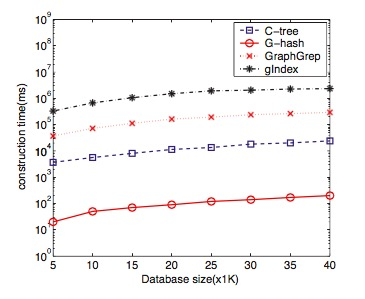
\includegraphics[width=\textwidth]{it}
        \caption{索引构造时间对比图}
        \label{fg:bb}
    \end{minipage}%
    \begin{minipage}[t]{0.5\textwidth}
        \centering
        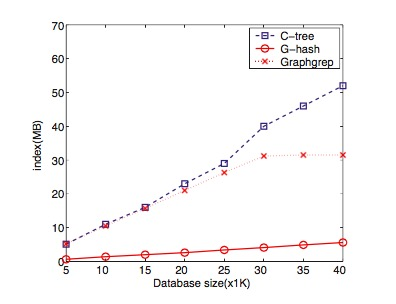
\includegraphics[width=\textwidth]{is}
        \caption{索引大小对比图}
        \label{fg:bi}
    \end{minipage}
\end{figure}

可以看出,无论构建时间,还是索引大小,G-Hash算法均优于其他算法。
\subsection{查询时间 \\ Query Processing Time}
我们探究了不同数据库大小对查询时间的影响,实验结果如图\ref{fg:ee}所示。
\begin{figure}[!ht]
    \centering
    \begin{minipage}[t]{0.5\textwidth}
        \centering
        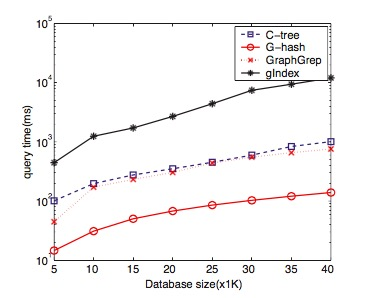
\includegraphics[width=\textwidth]{qt}
        \caption{查询时间和数据库大小关系对比图}
        \label{fg:ee}
    \end{minipage}%
    \begin{minipage}[t]{0.5\textwidth}
        \centering
         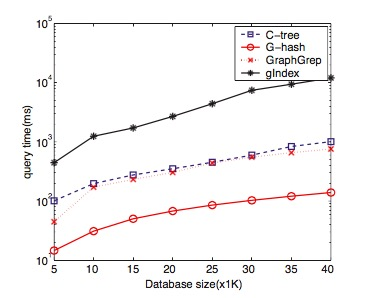
\includegraphics[width=\textwidth]{qt}
        \caption{查询时间和k值关系对比图}
        \label{fg:ek}
    \end{minipage}

\end{figure}

显然,G-Hash比其他算法表现均好,当数据库达到4000时,C-tree,GraphGrep和gIndex的查询时间是G-Hash的8倍,10倍和100倍。

最后我们比较了不同k值下查询时间,如图\ref{fg:ek}所示。


实验表明G-Hash的查询时间与k值的大小没有影响。

\ifx\allfiles\undefined
%\renewcommand\refname{参考文献}
%\bibliographystyle{unsrt}
%\bibliography{G-Hash翻译}
\end{document}
\fi
\ifx\allfiles\undefined
\documentclass{article}
\usepackage{amsmath}%换行
\usepackage{ctex}
\usepackage{tikz}
\usepackage{subfigure}
\usepackage{graphicx}
\usepackage{caption}
\usepackage{amsfonts, amssymb}%数学字体

\usepackage{indentfirst} %首行缩进
\makeatletter
\newcommand\figcaption{\def\@captype{figure}\caption} 
\newcommand\tabcaption{\def\@captype{table}\caption}
\renewcommand\figurename{图表} 
\makeatother
\usepackage{float}

\begin{document}

\else

\fi
\section{总结与展望}
图作为一种通用的数据结构已被广泛运用于大量领域,像化学分子学,生物信息学等等。大量知名学者当前都专注于数据管理方法和数据挖掘技术。而如何提出一种有效的图相似性搜索方法一直是一个重大的难题,因为现在大量算法都只专注于速度却不关心精确度。为了解决这个问题,我们提出了一种新的图查询算法G-Hash。通过我们的实验研究,我们在构造时间和效率上都明显有优势,这表明G-Hash已经可以支持大规模图数据库搜索。
\section{致谢}
感谢H.He和A.K.Singh提供C-tree源代码。感谢D.Shasha,J.T.L.Wang和R.Giugno提供的GraphGrep。感谢X.Yan,P.S.Yu和J.Han提供GIndexy源代码。我们的所有工作均是在KU中心支持下完成的,对他们表示由衷的感谢。
\ifx\allfiles\undefined
%\renewcommand\refname{参考文献}
%\bibliographystyle{unsrt}
%\bibliography{G-Hash翻译}
\end{document}
\fi


\bibliographystyle{unsrt}
\bibliography{G-Hash翻译}
\end{document}
